\section{Hosten auf einer Cloud}

Bisher zu diesem Zeitpunkt wurde die Applikation immer lokal ausgeführt. 
Dies führte zu einer Optimierung auf den regelmäßig verwendeten Geräten, jedoch zu Problemen bei neuen, aufgrund der benötigten Installationen und Einrichtung der benutzten Technologien. 
Ein einfacher Startvorgang des Projektes benötigt Java, Maven, PostgreSQL, Angular und der node package Manager.
Das erschwert die Nutzung der Applikation. 

Ebenso benötigt jeder Interessierte einen Zugang auf die GitHub Repositories, welche privat gestellt sind. 
Um das Projekt nun für jeden zur Verwendung zu stellen, muss dieses online verfügbar gemacht werden. 

\subsection{Vorbereitung}

Bevor die Applikation hochgeladen werden kann, müssen einige Änderungen am Code vorgenommen werden. 
Zum einen muss in den \emph{application.properties} einiges für die Production festgelegt werden. 
Die Datenbankwerte müssen den Konfigurationen des PostgreSQL-Services entsprechen. 
Genauso muss der Pfad für die Dateiverwaltung definiert werden auf der Cloud.
Zeile 7 legt den Uploadpfad der Dateien fest.
\begin{lstlisting}[label=lst:dbconfProd, caption=application.properties für Produktion]
%prod.quarkus.datasource.jdbc.url=jdbc:postgresql://postgres:5432/demo
%prod.quarkus.datasource.username = demo
%prod.quarkus.datasource.password = demo
%dev.quarkus.hibernate-orm.database.generation=drop-and-create
%dev.quarkus.hibernate-orm.sql-load-script=import.sql
quarkus.container-image.name=3dserver
%prod.three-d.file.upload.path=/srv/upload/files/
\end{lstlisting}    

In dieser Arbeit wurde für das Deployment die LeoCloud verwendet. 
Als Schüler oder Schülerin der HTBLA Leonding kann diese nach simpler Registrierung ohne Zahlungsvorgang genutzt werden. 
Die Cloud nutzt hauptsächlich Kubernetes, wodurch eine Installation der zugehörigen \gls{cli} \emph{kubectl} fundamental ist. 

Die LeoCloud verfügt über ihr eigenes Login Portal. 
Nach erfolgreicher Anmeldung wird eine Startseite angezeigt mit einem Bereich namens \emph{Mein Konto}. 
Dieser bildet den Namen des Namespaces ab, den Download eines demonstrativen Services, sowie andere Informationen. 
Der wichtigste Teil dieses Fensters ist der Button \emph{Mein Dashboard}. 

\begin{figure}
    \centering
    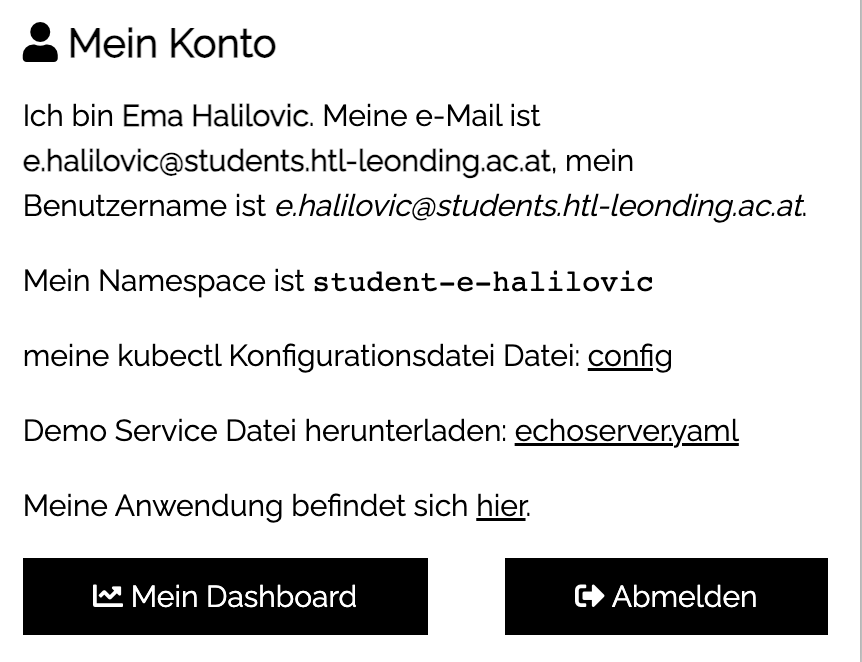
\includegraphics[scale=0.5]{pics/leowikimeinkonto.png}
    \caption{Persönlicher Bereich in der LeoCloud}
    \label{fig:implementation:meinkonto}
\end{figure}

Nach dessen Betätigung wird ein weiteres Fenster ersichtlich, was ein kurzes Tutorial anzeigt, wie auf das Dashboard zugegriffen werden kann. 
Das Kontrollzentrum lässt sich nur anzeigen, wenn im Terminal der Befehl aus \ref{lst:kubectlproxy} ausgeführt wurde. 
Da noch kein Upload Versuch durchgeführt wurde, zeigt das Dashboard anfangs keine relevanten Informationen.

\begin{lstlisting}[label=lst:kubectlproxy, language=bash, caption=Ausführung des Proxys für Kubernetes]
kubectl proxy
\end{lstlisting}    

Neben der Vorbereitung des Dashboards, wird ebenso ein GitHub Token für die Nutzung des \gls{ghcr} benötigt.
Dieser wird erstellt in den Developer Settings der Accounteinstellungen. 
Nach einer erfolgreichen zwei-faktor-Authentifizierung, können nun alle Rechte des Tokens angegeben werden. 
Für diesen Fall werden nur die in Abbildung \ref{fig:implementation:githubtoken} rosa eingerahmten Berechtigungen benutzt.

\begin{figure}
    \centering
    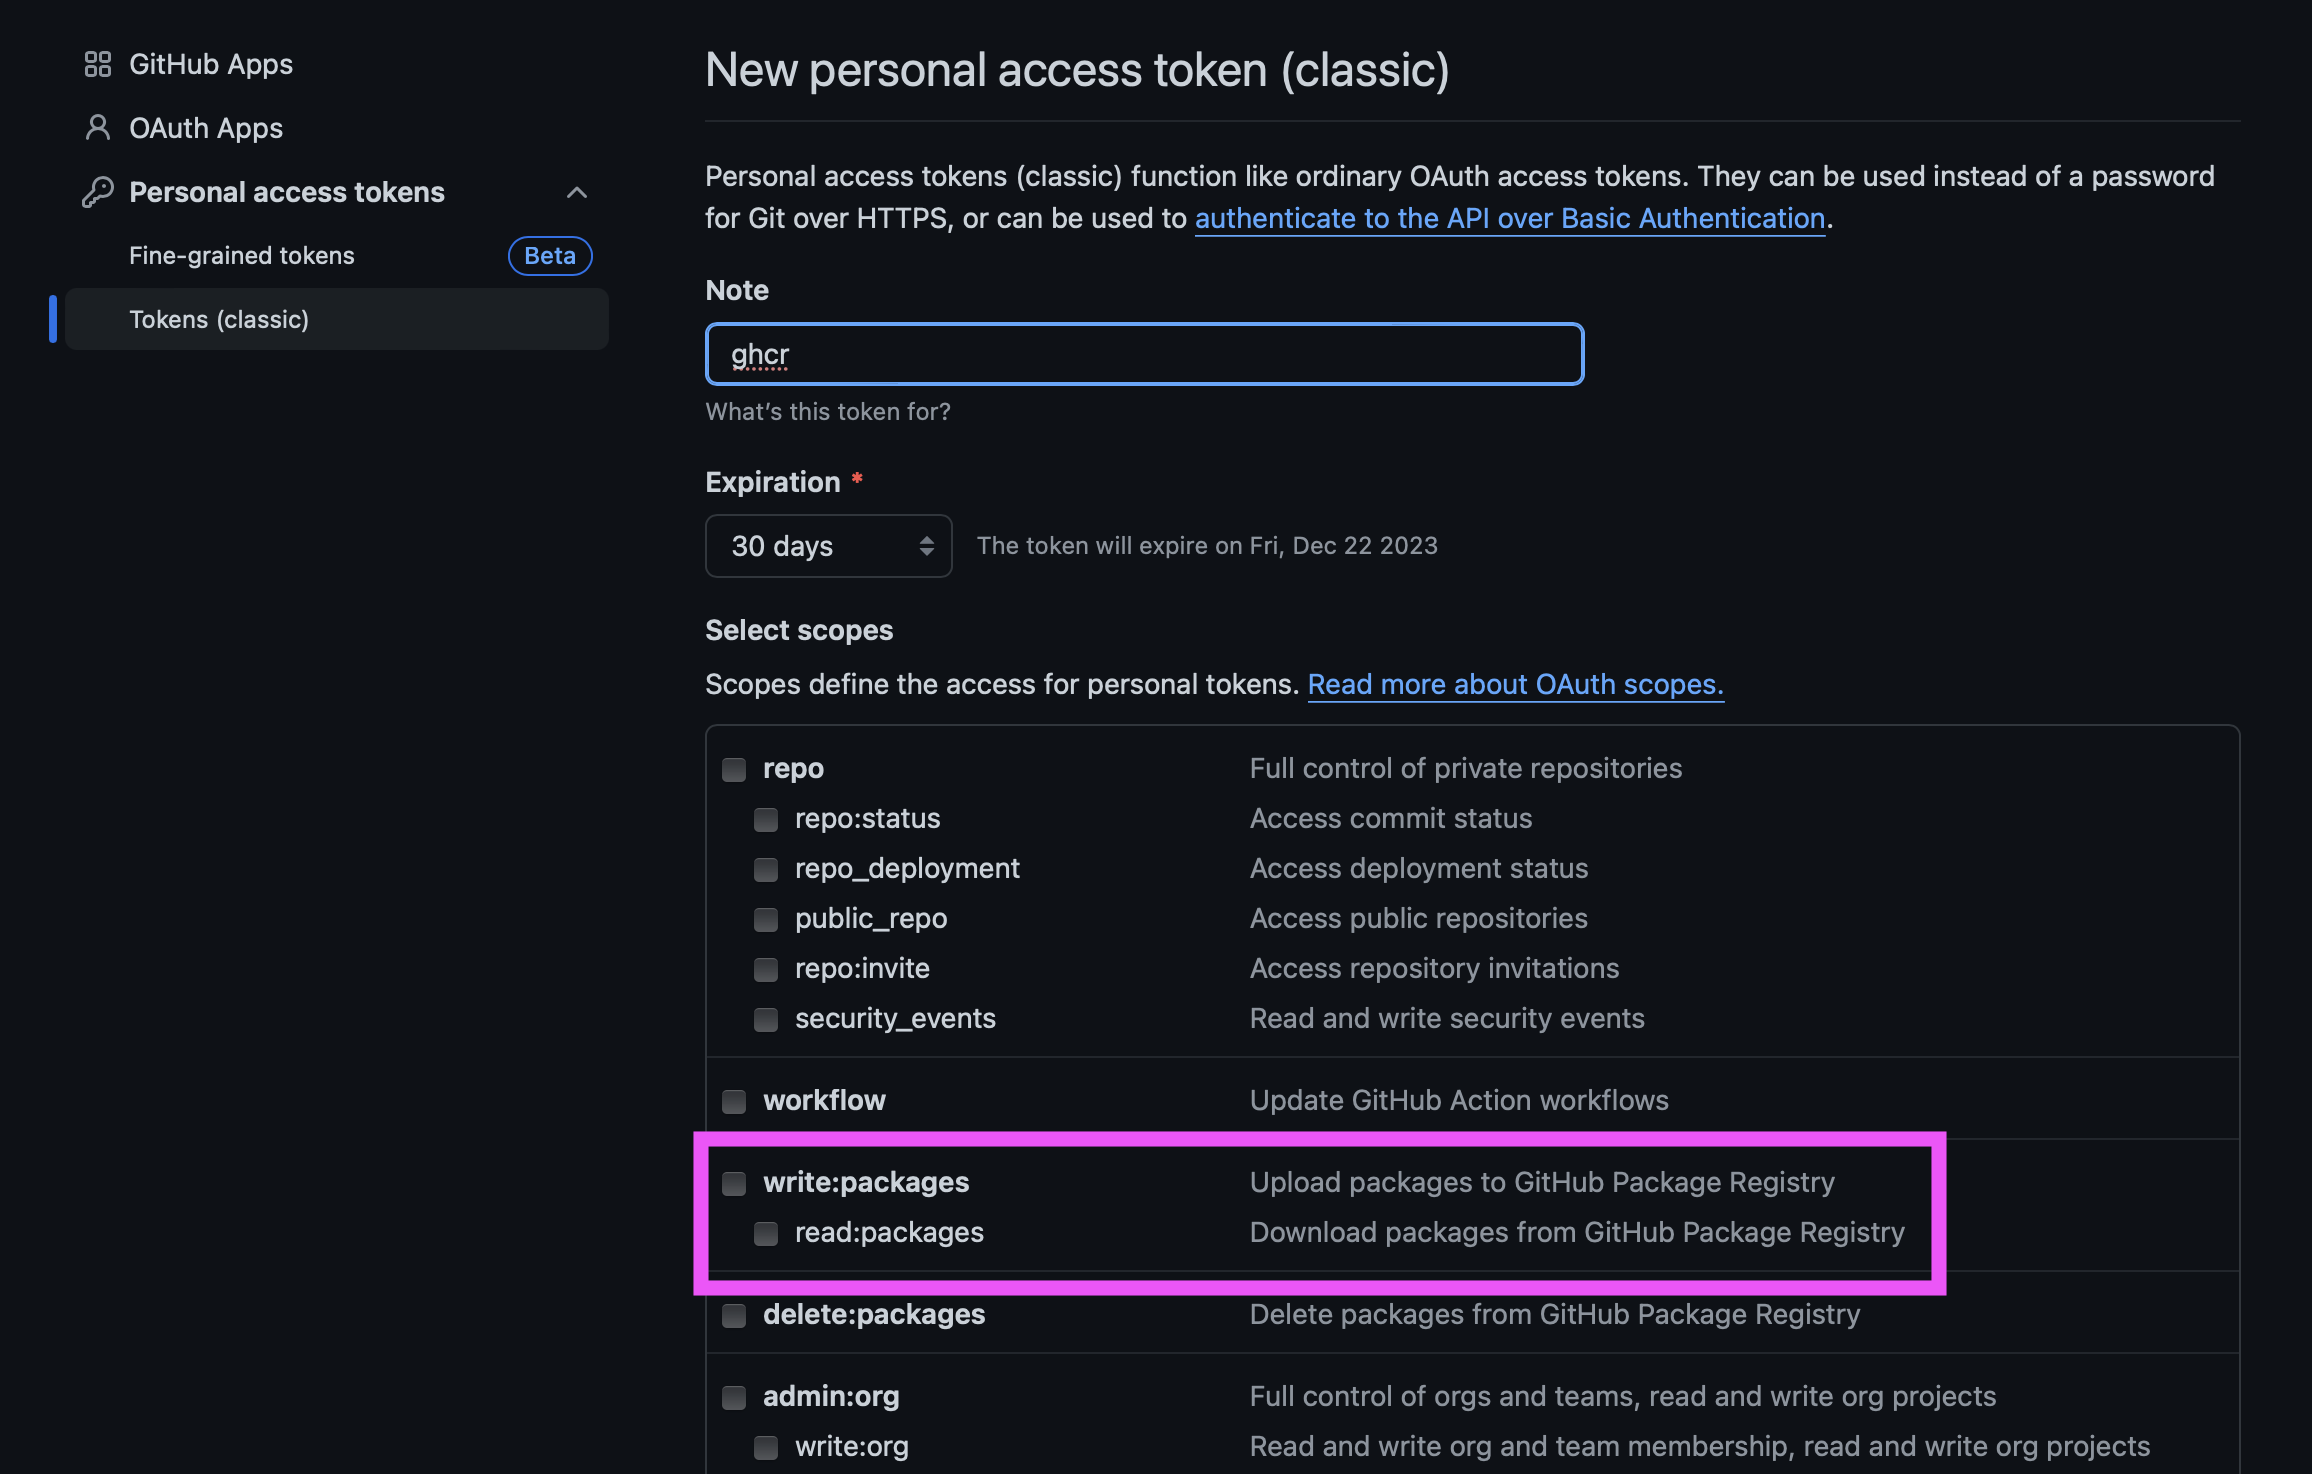
\includegraphics[scale=0.35]{pics/newtoken.png}
    \caption{Erstellung eines neuen Tokens}
    \label{fig:implementation:githubtoken}
\end{figure}

Nach Erstellung wird im Terminal Befehl \ref{lst:loginghcr} eingegeben. 
Im Terminal werden dann die weiteren Schritte beschrieben (siehe Abb. \ref{fig:implementation:githublogin}). 
Bei der Passwortanforderung muss der in GitHub erstellte Token angegeben werden. 
Wichtig ist zu beachten, dass Docker am Gerät gestartet sein muss. 

\begin{figure}
    \centering
    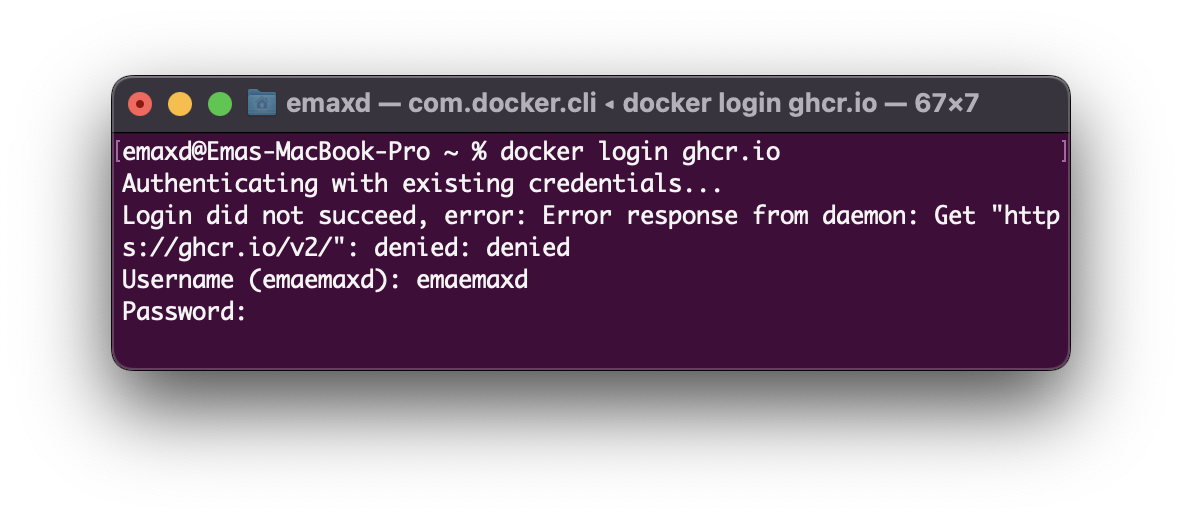
\includegraphics[scale=0.5]{pics/ghcrloginterminal.png}
    \caption{Login für das GHCR}
    \label{fig:implementation:githublogin}
\end{figure}

\begin{lstlisting}[label=lst:loginghcr, language=bash, caption=GHCR Login]
docker login ghcr.io
\end{lstlisting}
\subsection{Umsetzung}

Dafür wurde ein Ordner aus dem Unterricht mit Herr Christian Aberger als Vorlage genommen namens \emph{k8s}. 
In diesem waren allgemeine Dateien, wie \emph{namespace.yaml}, schon angelegt, jedoch waren Anpassungen noch benötigt. 
Der Codeblock aus \ref{lst:namespaceyaml} zeigt den ganzen Inhalt dieses Files an. 
In dem vorher erwähnten File wird Zeile 4 in \ref{lst:namespaceyaml} mit dem angezeigten Namespace aus Abbildung \ref{fig:implementation:meinkonto} ersetzt. 
\begin{lstlisting}[label=lst:namespaceyaml, language=bash, caption=Namespace konfiguration in namespace.yaml]
apiVersion: v1
kind: Namespaces
metadata:
  name: student-e-halilovic
\end{lstlisting}

Das Hauptelement des Deployments ist das \emph{build.sh}-File. 
Es wird im Projekt-Root-Verzeichnis angelegt, da es durch die zentrale Position auf alle Ordner einfach zugreifen kann. 
In dieser Datei werden Prozesse für den Upload, sowie dafür benötigte Variablen, definiert. 
Wichtig sind Variablen, die den kompletten Namen des Packages definieren, sowie den GitHub-User. 
Dabei muss beachtet werden, dass Docker-Packagenamen keine Großbuchstaben enthalten dürfen. 
Um die Variablen für andere Skripten zur Verfügung zu stellen, werden diese exportiert. 
Die Umsetzung dieses Prozesses erfolgt durch die Befehle in Codeausschnitt \ref{lst:buildshanfang}.

\begin{lstlisting}[label=lst:buildshanfang, language=bash, caption=Anfang der build.sh-Datei]
BASE_HREF=${BASE_HREF:-"/e.halilovic/"}
GITHUB_USER=${GITHUB_USER:-emaemaxd}
BACKEND_IMAGE_NAME=ghcr.io/$LC_GH_USER_NAME/3dserver:latest
export GITHUB_USER
export BACKEND_IMAGE_NAME
\end{lstlisting}    

Nachdem die Hauptkonfiguration definiert wurde, können nun die Hauptkomponenten Schritt für Schritt für den Upload vorbereitet werden. 
Zuerst wird mit dem Befehl \emph{pushd} der aktuelle Pfad in den Verzeichnisstapel gelegt und in die Quarkus-Anwendung hineingewechselt. 
Anschließend wird die Applikation mit Maven in ein Package kompiliert und in einen neuen Ordner hineinkopiert. 
Mithilfe von Docker wird nach diesem Schritt ein Image erstellt unter dem Namen \emph{3dserver}. 
Dieses wird von Docker benutzt, um ein weiteres Image zu erzeugen, nur dieses Mal unter dem Namen der vorher definierten Variable \emph{BACKEND\_IMAGE\_NAME} (siehe Abb. \ref{lst:buildshanfang} Zeile 6). 
Zuletzt wird das Image auf das \gls{ghcr} gepusht und der Pfad des Shell-Skripts auf den Ausgangswert zurückgesetzt. 
Dies alles beschreibt die Befehle in Codeausschnitt \ref{lst:buildshquarkus}.

\begin{lstlisting}[label=lst:buildshquarkus, language=bash, caption=Quarkus-Teil in der build.sh-Datei]
pushd server/three-d-portfolio-server
mvn clean package
mkdir -p target/deploy
cp target/*-runner.jar target/deploy/
docker build --tag 3dserver --file ./src/main/docker/Dockerfile ./target/deploy
docker image tag 3dserver $BACKEND_IMAGE_NAME
docker push $BACKEND_IMAGE_NAME
popd
\end{lstlisting}

Danach wird die Angular-Applikation vorbereitet. 
Hier wird ebenso in das dafür zugehörige Verzeichnis gewechselt.
Mittels dem node package Manager werden alle Abhängigkeiten installiert, bevor die Anwendung gestartet wird. 
Der Befehl in Codeabschnitt \ref{lst:buildshangular} Zeile 3 konfiguriert zusätzlich noch, dass mit Produktionskonfiguration gearbeitet werden soll. 
Ebenso wird definiert, unter welchem Pfad die Anwendung verfügbar sein wird.

\begin{lstlisting}[label=lst:buildshangular, language=bash, caption=Frontend-relevanter Teil der build.sh-Datei]
pushd 3D-Portfolio-Gallery/Gallery
npm install
npm run build -- --configuration production --base-href $BASE_HREF
popd
\end{lstlisting}

Nachfolgend wird das \emph{deploy.sh}-File im \emph{k8s}-Ordner (siehe Codeabschnitt \ref{lst:deploy:k8s}) ausgeführt. 
Diese definiert gleich in Zeile 1, dass nach einem Fehler das Skript abgebrochen werden soll. 
Zeile 3 sorgt dafür, dass die Variable durch ihren tatsächlichen Wert ersetzt wird. 
Die nachfolgenden Befehle legen Konfigurationen für den Kubernetes-Cluster fest.

\begin{lstlisting}[label=lst:deploy:k8s, language=bash, caption=k8s deploy.sh-Datei]
set -e
mkdir -p target
envsubst '\$BACKEND_IMAGE_NAME' < appsrv.yaml > ./target/appsrv.yaml
kubectl delete -f appsrv.yaml || echo "appsrv not deployed yet"
# ...
kubectl apply -f busybox-job.yaml
kubectl apply -f ingress.yaml || echo "no ingress"
kubectl rollout restart deployment/nginx || echo "no nginx yet"
kubectl rollout restart deployment/appsrv || echo "no appsrv yet"
\end{lstlisting}

Die angewendeten Dateien enthalten alle näheren Konfigurationen für die einzelnen Pods. 
Der unten angeführte Codeblock stammt aus der \emph{appsrv.yaml}-Datei, die sehr relevant ist für die Erstellung des Quarkus Applikationsserver. 
In ihr definiert man unter anderem, welches Image gezogen werden soll, unter welchem Pfad die Dateien gesichert werden, sowie unter welchem Port die Anwendung erreichbar ist.
Das Image, welches in der Variable \emph{BACKEND\_IMAGE\_NAME} steht, wird bei Ausführung der \emph{build.sh}-Datei das Package privat auf GitHub hochgeladen.
Damit der Applikationsserver darauf zugreifen kann, muss es jedoch manuell in den Packagesettings veröffentlicht werden (siehe Abb. \ref{fig:implementation:3dserverpackage}).

\begin{lstlisting}[label=lst:yaml:appsrv, language=bash, caption=Ausschnitt aus appsrv.yaml-Datei]
    apiVersion: apps/v1
    kind: Deployment
    metadata:
      name: appsrv
      namespace: student-e-halilovic
    spec:
      replicas: 1
      selector:
        matchLabels:
          app: appsrv
      template:
        metadata:
          labels:
            app: appsrv
        spec:
          containers:
            - name: appsrv
              image: $BACKEND_IMAGE_NAME
              imagePullPolicy: Always
              ports:
                - containerPort: 8080
              volumeMounts:
                - name: upload
                  mountPath: /srv/upload
          volumes:
            - name: upload
              persistentVolumeClaim:
                claimName: appsrv-upload
    ---
    apiVersion: v1
    kind: Service
    metadata:
      name: quarkus
      namespace: student-e-halilovic
    spec:
      ports:
        - port: 8080
          targetPort: 8080
          protocol: TCP
      selector:
        app: appsrv
\end{lstlisting}

\begin{figure}
    \centering
    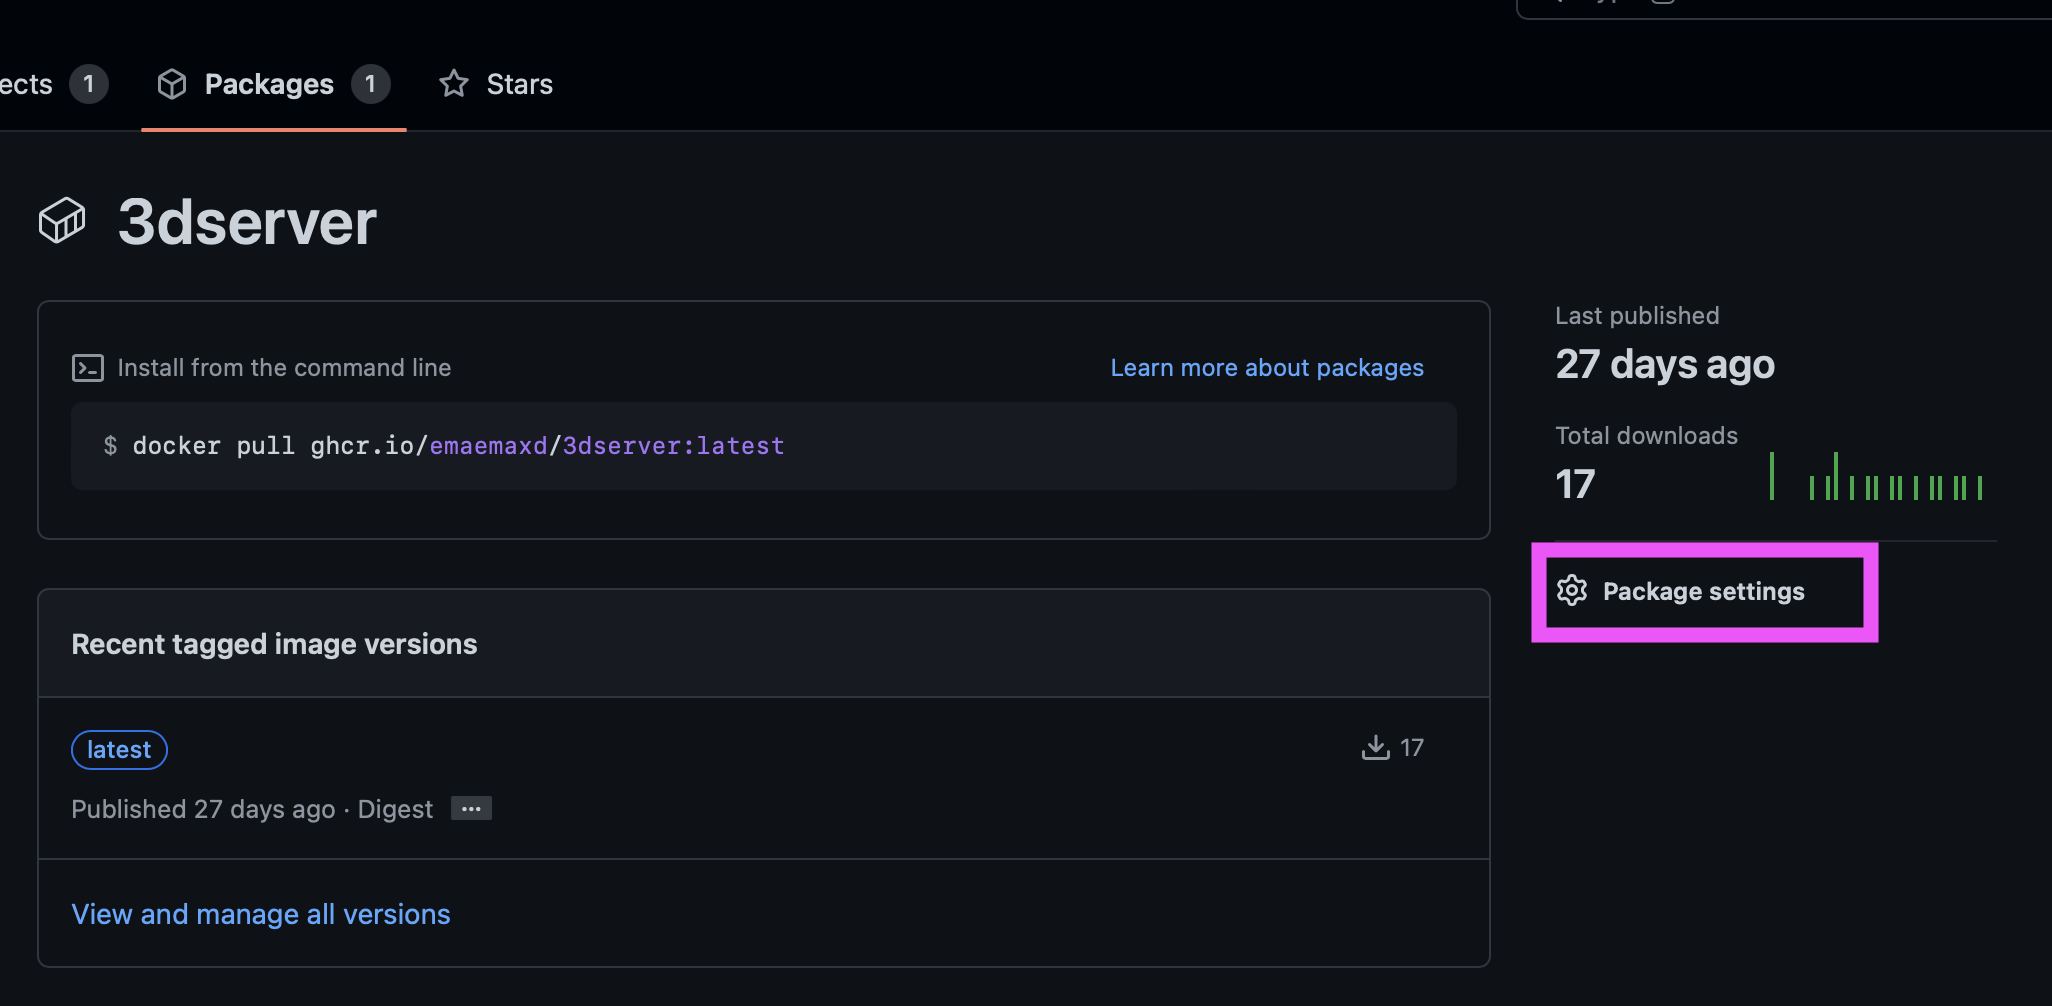
\includegraphics[scale=0.5]{pics/3dserverpackage.png}
    \caption{Ansicht des erstellten Packages in GitHub}
    \label{fig:implementation:3dserverpackage}
\end{figure}

Für Angular wird ein nginx-Server benötigt. 
Dieser hostet das Frontend und leitet die Requests an die Quarkus Anwendung weiter. 
Anfangs sieht das \emph{nginx.yaml}-Skript dem \emph{appsrv.yaml} ähnlich, jedoch wird am Ende noch ein Proxy eingerichtet.

\begin{lstlisting}[label=lst:yaml:nginx, language=bash, caption=Ausschnitt aus nginx.yaml-Datei]
# ...
data:
    default.conf: |
    server {
        listen 80;
        rewrite_log on;
        error_log /dev/stdout debug;
        root /usr/share/nginx/html/gallery;
        index index.html;
        try_files $uri $uri/ /index.html =404;
        
        location /api/ {
            proxy_pass http://quarkus:8080;
            proxy_set_header X-Forwarded-For $proxy_add_x_forwarded_for;
            proxy_set_header X-Real-IP $remote_addr;
            proxy_set_header Host $host:$server_port;
        }
    }
\end{lstlisting}

Nach dem Skript wird eine Funktion aufgerufen, die auf den Start des Pods wartet. 
Dies geschieht durch die Ausführung eine Schleife, die in jedem Durchgang überprüft, ob ein Wert in der Variable \emph{KNIFE\_POD} steht.
Falls nicht, kommt es zu einem neuen Durchgang, wobei die Variable neu geschrieben, sodass die Schleife nicht endlos läuft. 
Ebenso wird bei jeder Runde für eine Sekunde gewartet.
Dies geschieht durch den Befehl in Zeile 3 in Codeausschnitt \ref{lst:buildsh:knife}. 
Hier werden die Pods wiedergegeben und zurechtgeschnitten, sodass sie am Ende in der Variable exportiert werden.  

\begin{lstlisting}[label=lst:buildsh:knife, language=bash, caption=Knife-Funktion in der build.sh-Datei]
KNIFE_POD=""
findPod() {
    KNIFE_POD=$(kubectl -n $NAMESPACE get pods|grep -i Running|grep knife|cut -d\  -f 1)
}
waitForPod() {
    local pod=""
    while [ "$KNIFE_POD." == "." ]; do
        findPod $1
        kubectl -n $NAMESPACE get pods | grep knife
            echo "wait for knife"
            sleep 1
    done;
}
waitForPod knife
export KNIFE_POD
export NAMESPACE
\end{lstlisting}

Nach dieser Funktion wird im Angular-Verzeichnis die \emph{deploy.sh}-Datei ausgeführt. 
Diese Kopiert das dist-Verzeichnis auf den Namespace Pod. 

\begin{lstlisting}[label=lst:deploy:angular, language=bash, caption=deploy.sh-Datei für Angular]
set -e
kubectl -n $NAMESPACE  exec $KNIFE_POD -- rm -rf /srv/demo /srv/dist
pushd ./dist
    kubectl -n $NAMESPACE  cp * $KNIFE_POD:/srv/
popd
\end{lstlisting}

Nach Angular werden die Quarkus Dateien auf den Namespace geladen.

\begin{lstlisting}[label=lst:deploy:angular, language=bash, caption=Kopieren der Datei für Quarkus]
pushd server/three-d-portfolio-server/target
kubectl -n $NAMESPACE cp files/ $KNIFE_POD:/mnt/
popd
\end{lstlisting}

Der letzte Befehl löscht die Resource \emph{busybox-job.yaml} aus dem Kubernetes-Cluster, die in Codeabschnitt \ref{lst:deploy:k8s} definiert wurde. 

\begin{lstlisting}[label=lst:deploy:angular, language=bash, caption=letzter Befehl der build.sh-Datei]
kubectl delete -f busybox-job.yaml
\end{lstlisting}